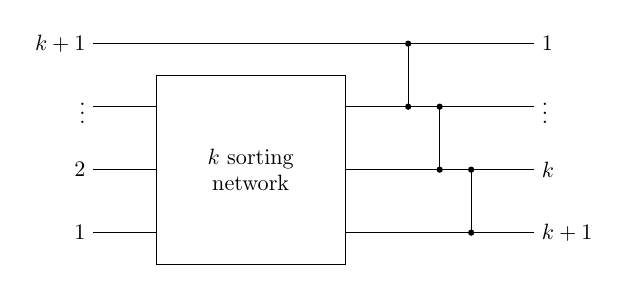
\begin{tikzpicture}[scale=0.8,every node/.style={scale=0.8}]
\tikzstyle{bdot} = [fill=black,circle,scale=0.3];
\draw  (-2.5,0) node[left] {$k+1$} -- (4.5,0) node[right] {$1$};
\draw (-2.5,-1) node[left] {$\vdots$}-- (4.5,-1) node[right] {$\vdots$};
\draw (-2.5,-2) node[left] {$2$}-- (4.5,-2) node[right] {$k$};
\draw (-2.5,-3) node[left] {$1$}-- (4.5,-3) node[right] {$k+1$};

\draw[fill=white]  (-1.5,-0.5) rectangle (1.5,-3.5);
\node[text width=2cm,text centered] at (0,-2) {$k$ sorting network};
\draw (2.5,0) node [bdot] {} -- (2.5,-1) node [bdot] {};
\draw (3,-1) node [bdot] {} -- (3,-2) node [bdot] {};
\draw (3.5,-2) node [bdot] {} -- (3.5,-3) node [bdot] {};




\end{tikzpicture}
